\documentclass{standalone}
\usepackage{tikz}
\begin{document}
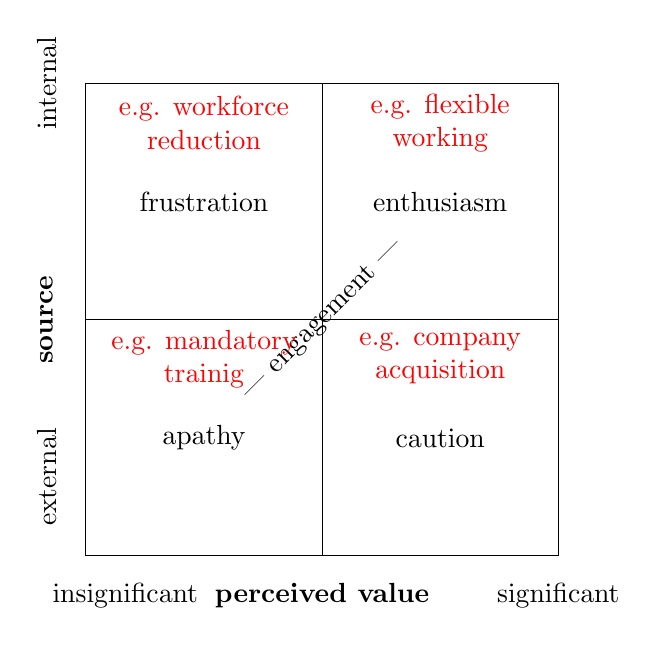
\begin{tikzpicture}
    \draw (0,0) rectangle (6,6) ;
    \draw (0,3) -- (6,3) ;
    \draw (3,0) -- (3,6);
    \node[rotate=90] at (-0.5,3) {\textbf{source}};
    \node at (3,-0.5) {\textbf{perceived value}};
    
    \node at (0.5,-0.5) {insignificant};
    \node at (6,-0.5) {significant};
    
    \node[rotate=90] at (-0.5,1) {external};
    
    \node[rotate=90] at (-0.5,6) {internal};

    \node[rotate=45] at (3,3) {--- engagement --- };
    
    \node at (1.5,4.5) {frustration};
        \node[red] at (1.5,5.5) {\parbox{2.5cm}{\centering e.g. workforce reduction}};
    \node at (4.5,4.5) {enthusiasm};
        \node[red] at (4.5,5.5) {\parbox{2.5cm}{\centering e.g. flexible working}};
    \node at (1.5,1.5) {apathy};
        \node[red] at (1.5,2.5) {\parbox{2.5cm}{\centering e.g. mandatory trainig}};    
    \node at (4.5,1.5) {caution};
        \node[red] at (4.5,2.5) {\parbox{2.5cm}{\centering e.g. company acquisition}};        
\end{tikzpicture}

% Source: \cite[p. 37]{Roberts}

\end{document}